\chapter{Introduction}\label{introduction}

\section{Background and Motivation}

The CESAR project aim to use low cost sensor kit to prototype applications using physiological signals related to heart rate, brain activity, oxygen level in blood to monitor sleep and breathing related illnesses, like Obstructive Sleep Apnea (OSA). Side effects of OSA do not only cause sleepiness during day time (which might affect daily chores), but also serious illnesses like diabetes and cardiac dysfunctions. Statistically speaking, it is estimated that about 25\% of the adult population in Norway has OSA, but only 10\% of them are diagnosed. A major problem with diagnosing OSA is polysomnography in \textit{sleep laboratories} \cite{cesar}. This is both really expensive and inefficient due to lacking capacity to perform sufficient tests with patients. Hence, the CESAR project aims to contribute to this situation with a low-cost Android and BiTalino based system to tackle these problems in a minimal invasive approach. 

The project has been developed by various people over the years, and the system has been divided into three parts (illustrated in Figure \ref{fig:parts}). The data acquisition part, the data streams dispatching part, and the application part. The first two parts are already implemented (summarized in the section below), thus, the last part is what we will be focusing throughout this thesis. 

\begin{figure}
    \centering
    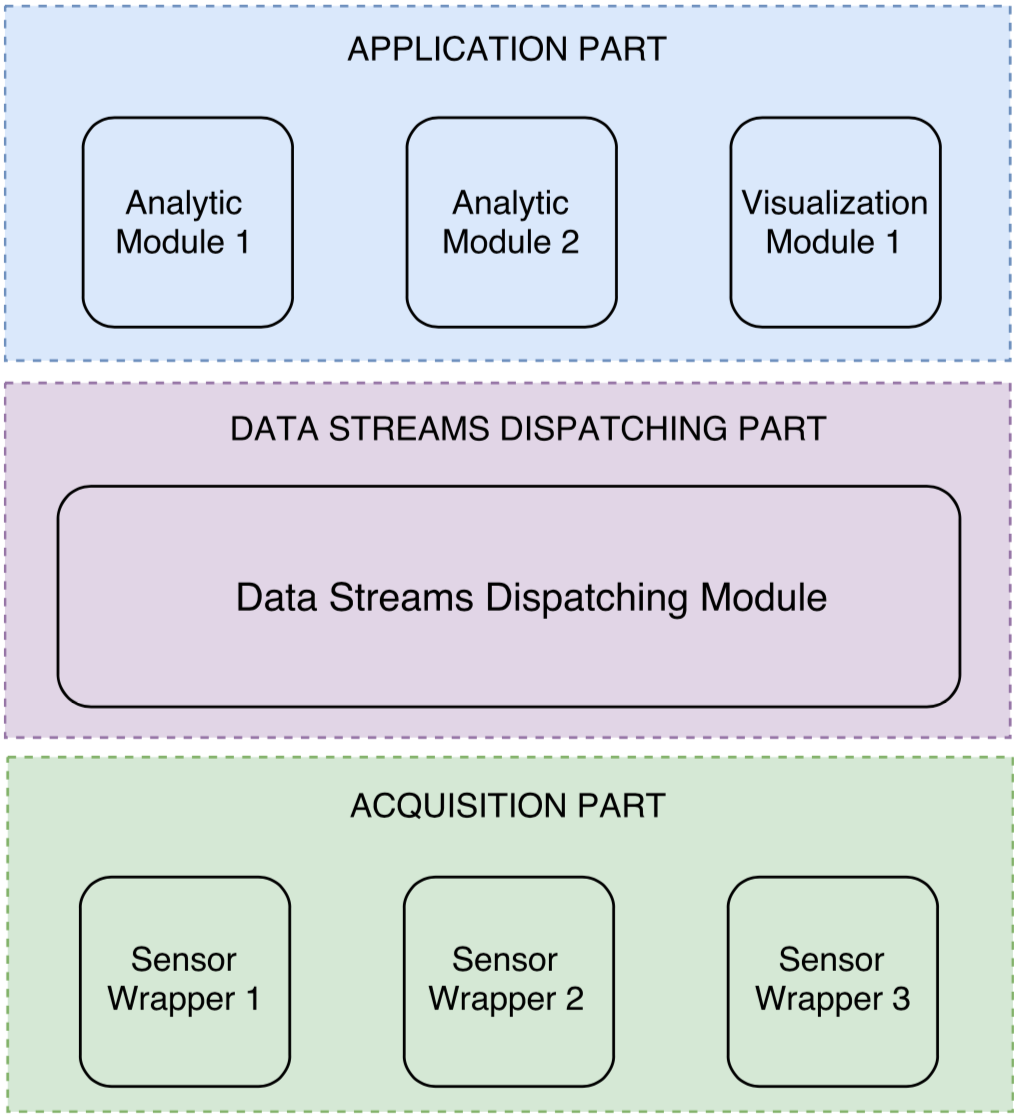
\includegraphics[width=0.5\textwidth]{images/parts.png}
    \caption{Structure of the project, separating functionality into three independent layers \cite{daniel}}
    \label{fig:parts}
\end{figure}

\section{Problem Statement}

The market has new and affordable sensors that can aid with the data acquisition, which we seamlessly can integrate with the extensible data streams dispatching tool. The Flow sensor is an interesting sensor source due to its versatility and adaptability of collecting breathing data and connecting to devices with the BlueTooth protocol. 

As for the state of this thesis: (i) applications which supports the Flow sensor has not been designed for end-users, in essence, they provide no user-friendly interface that allows for sharing of the data. In order to extract the data from these applications, the mobile device has to be connected with a PC over USB for data transfer; (ii) there is no sensor wrappers that support the Flow sensor with the data streams dispatching tool in the CESAR project; and (iii) the data streams dispatching tool is not ready to be used by the end-users, because the project facilitates no user-friendly interface for users to record the data from the supported sensor sources.

As such, we look into designing and implementing an Android application (Nidra) that record, share, and analyze breathing data over an extended period (e.g., during sleep) by using the Flow sensor. Additionally, we want to facilitate an extensible application such that future developers can extend functionality or enrich the data in Nidra. In the end, we can hopefully strengthen the analysis of abnormal sleeping patterns to decreasing the risk of the symptoms they may come as a consequence. Also, as a bi-product, the application can be used in other fields of studies (e.g., physical activities). As the scope of this thesis, we focus on the completion of three main goals:

\begin{description}
    \item[Goal 1] Integrate the support for Flow sensor by creating a sensor wrapper that connects with the extensible data streams dispatching tool.
    \item[Goal 2] Research and develop a user-friendly application which facilitates collection of breathing data with the Flow sensor, sharing of the data, and analysis of the data with the use of the extensible data streams dispatching tool.
    \item[Goal 3] Create an extensible solution such that the developers can create standalone applications that integrate with Nidra. 
\end{description}

As part of the goals of this thesis, we also define three system requirements to keep in mind while designing and implementing the application. The three system requirements are the following: 

\begin{description}
    \item[Requirement 1] The application must provide an interface for the patient to (i) record physiological signals (e.g., breathing data); (ii) present the results; and (iii) share the results.
    \item[Requirement 2] The application must ensure that upon sensor disconnections, the connectivity is reinstated to minimize the data loss and its effects on the data analysis.
    \item[Requirement 3] The application must provide an interface for the developers to create modules that integrate with the application.
\end{description}



\section{Limitations}
Based on the goals and requirements stated in the previous section, the scope of this thesis is to design and implement an application capable of recording breathing data obtained by the Flow sensor over an extended period. 

We limit the scope to integrating the support for the Flow sensor in Nidra, and excluded to test for already integrated sensor sources (e.g., Bitalino). Further, with the Flow sensor provided under development, we restricted the design to collect respiration (breathing) data (as opposed to hearth-rate or other physiological data).

The application is designed to collect breathing data; we do not perform any analysis to predict or detect sleeping disorders based on the data. However, we facilitate for future developers to utilize the data provided by Nidra to perform such tasks.

Finally, the implementation is Android-specific as the previous work performed on the project is designed solely for Android applications. 

\section{Research Method}
The work in this thesis is classified as \textit{computing research} with a principle approach of an \textit{engineering method} as described in \cite{Glass_1995}. The engineering method (evolutionary paradigm) is to: (i) observe existing methods, (ii) propose a better solution, (iii)  build or develop artifacts\footnote{human-manufactured objects produced during the development}, and (iv) measure and analyze until no further improvements are possible. The report identifies patterns amongst various principle approaches and categorizes the the patterns into phases: \textit{(i) informational phase}, \textit{(ii) propositional phase}, \textit{(iii) analytical phase}, and \textit{(iv) evaluation phase}. Below, we give a brief description of each phase and discuss how our work fits into each of them. 

\subsection{Informational Phase}
The informational phase according to the report is to \textit{"gather or aggregate information via reflection, literature survey, people/organization survey, or poll"}

In this thesis, we survey previous related work in the field of detecting, analyzing, and diagnosing sleep related-breathing disorders on a mobile device. Based on this, we derive that the application created in this thesis tries to solve the same problem; however, the related work operates with different measure or instrument for solutions (e.g., using microphone and accelerometers to provide early-detection of sleep apnea). As such, we focused on creating an application that allows future developers to create modules on top of our solution (as illustrated in Figure \ref{fig:nidra_modules}). By allowing this, future developers can expedite the innovation in the research and study of sleep-related breathing disorders, as well as allowing the patients to operate with one application. 

\begin{figure}
    \centering
    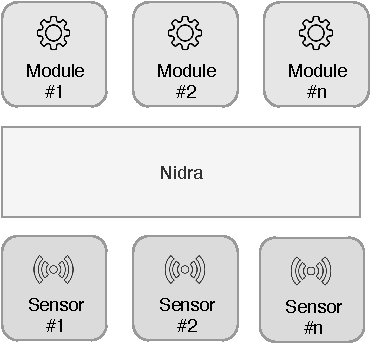
\includegraphics[scale=0.8]{images/Nidramodules.pdf}
    \caption{Nidra: operating with multiple modules that extends the functionality or provide data enrichiment, and integrating support for multiple sensor source (with the use of the data streams dispatching tool).}
    \label{fig:nidra_modules}
\end{figure}

\subsection{Propositional Phase}
The propositional phase according to the report is to \textit{"propose and/or formulate a hypothesis, method or algorithm, model, theory, or solution"}

The solution proposition in this thesis is to create an application used to record, share, and analyze breathing data collected over an extended period. We want to extend the CESAR project by providing an user-interface to the patient to perform these tasks while using the tools that the project facilitates. Mainly, we want to use the data streams dispatching tool in order to manage current and future sensor sources. In which, we proceed to add support for the Flow sensor. In the end, we wish to facilitate an application that is used by the patients to record their breathing data during sleep and to share the data between researchers/doctors. As such, we aid in analyzing the data to detect sleep-related breathing disorders (e.g., obstructive sleep apnea) from home. 

\subsection{Analytical Phase}
The analytical phase according to the report is to \textit{"analyze and explore a proposition, leading to a demonstration and/or formulation of a principle or theory"}

With the proposition phase of this thesis, we analyze the tasks of the application. We separate the tasks into concerns (i.e., recording, sharing, analyzing, modules, storage, and presentation) where we propose a structure that encompasses components with functionality and design choices. With each concern combined, we drive towards the fulfilling the goals of this thesis. As a demonstration, we realize the design choices by implementing them as an Android application, called Nidra. 

\subsection{Evaluation Phase}
The evaluation phase according to the report is to \textit{"evaluate a proposition or analytic finding by means of experimentation (controlled) or observation (uncontrolled, such as a case study or protocol analysis), perhaps leading to a substantiated model, principle, or theory"}

Based on the requirements and goal of this thesis, we evaluate the application by conducting experiments. Some of the experiments include participants that perform various tasks, such that we can observe the outcome of the tasks on participants without prior knowledge or experience of the application. In the end, we evaluate and conclude whether the goals and requirements of this thesis are sufficient.

\section{Thesis Outline}
The thesis is divided into three parts, which the following list presents a general overview of:

\begin{itemize}
    \item Part 1: \textbf{Introduction \& Background}
    \begin{description}[font=\normalfont\itshape]
        \item[Chapther 2: Background] presents the background material necessary for understanding the fundamentals of this thesis. It starts by introducing the CESAR project and the tools provided for data acquisition, as well as a description of the Flow sensor. Finally, an overview of the Android operating with the information required to understand the structure of the application (Nidra).
        \item[Chapther 3: Related Work] presents the related work focusing on creating a mobile application to collect physiological data in order to diagnose sleep apnea, and with a brief discussion on how we contribute with novelty and improvements from the related work.
    \end{description}

    \item Part 2: \textbf{Design \& Implementation}
    \begin{description}[font=\normalfont\itshape]
        \item[Chapther 4: Analysis and High-Level Design] presents the functional requirements of the application, the tasks derived based on the requirements and goals of the thesis, and the tasks separated into concerns, where we propose a structure of implementation which encompasses component with functionality and design choices. In the end, we discuss the data structure, namely the data entities (i.e., record, sample, module, and user), the data format (JSON versus XML), and the structure of the data packets sent from the sensor sources as well as the data packets sent on sharing. 
        \item[Chapther 5: Implementation] presents the application components of the project (i.e., Nidra, data streams dispatching module, and the Flow sensor wrapper) with the interface of IPC connectivity. Moreover, it presents the steps and flows taken in order to implement the concerns (i.e., recording, sharing, analyzing, modules, storage, and presentation) by separating the actions and showing how the components in the application interact.
    \end{description}

    \item Part 3: \textbf{Evaluation \& Conclusion}
    
    \begin{description}[font=\normalfont\itshape]
        \item[Chapther 6: Evaluation] presents four experiments conducted in order to evaluate the system requirements of the application.  Each experiment has a short description followed up by results, a discussion on improvements and findings, and a conclusion of the experiment. 
        \item[Chapther 7: Conclusion] presents the summary of the thesis, followed up with contributions that answer the goals defined in the problem statement.
    \end{description}

\end{itemize}



